\begin{frame}{Setups}
	\begin{figure} 
		\begin{center}
			\begin{subfigure}{0.45\textwidth}  
				\centering 
				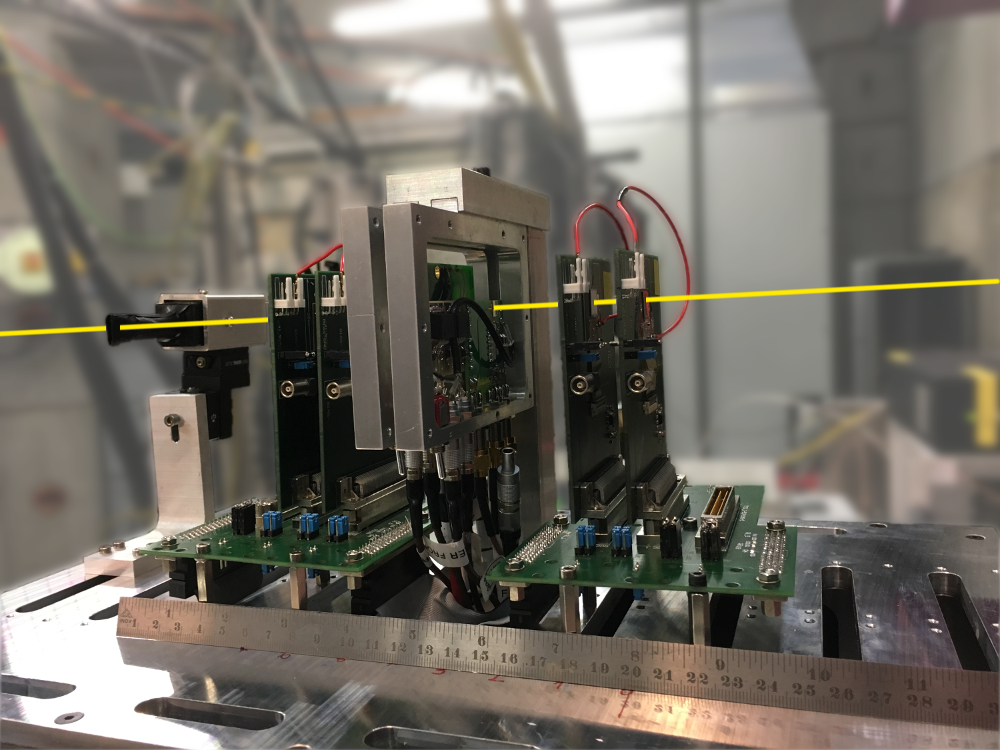
\includegraphics[height=.45\textheight]{TelPad}
				\caption{pad setup}
			\end{subfigure}
			\begin{subfigure}{0.45\textwidth} 
				\centering 
				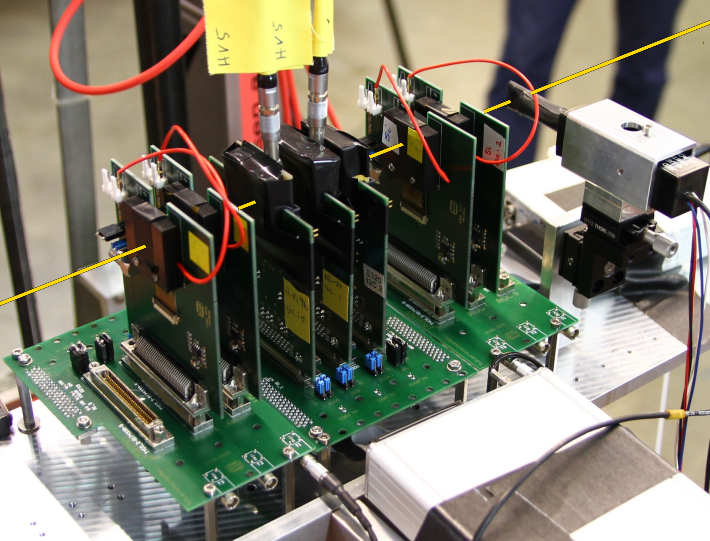
\includegraphics[height=.45\textheight]{TelPix}
				\caption{pixel setup} 	
			\end{subfigure} 
		\end{center}
	\end{figure}
	\vspace*{10pt}
	\begin{itemize}
		\item pad setup: testing whole diamond as a single readout device
		\item pixel setup: testing diamond as sensor material on CMS-Pixel Chips
	\end{itemize}
\end{frame}
% ===================== FRAME 7 ===========================================
\subsection{Module}
\begin{frame}{Telescope Module}
	\begin{figure}
		\centering
		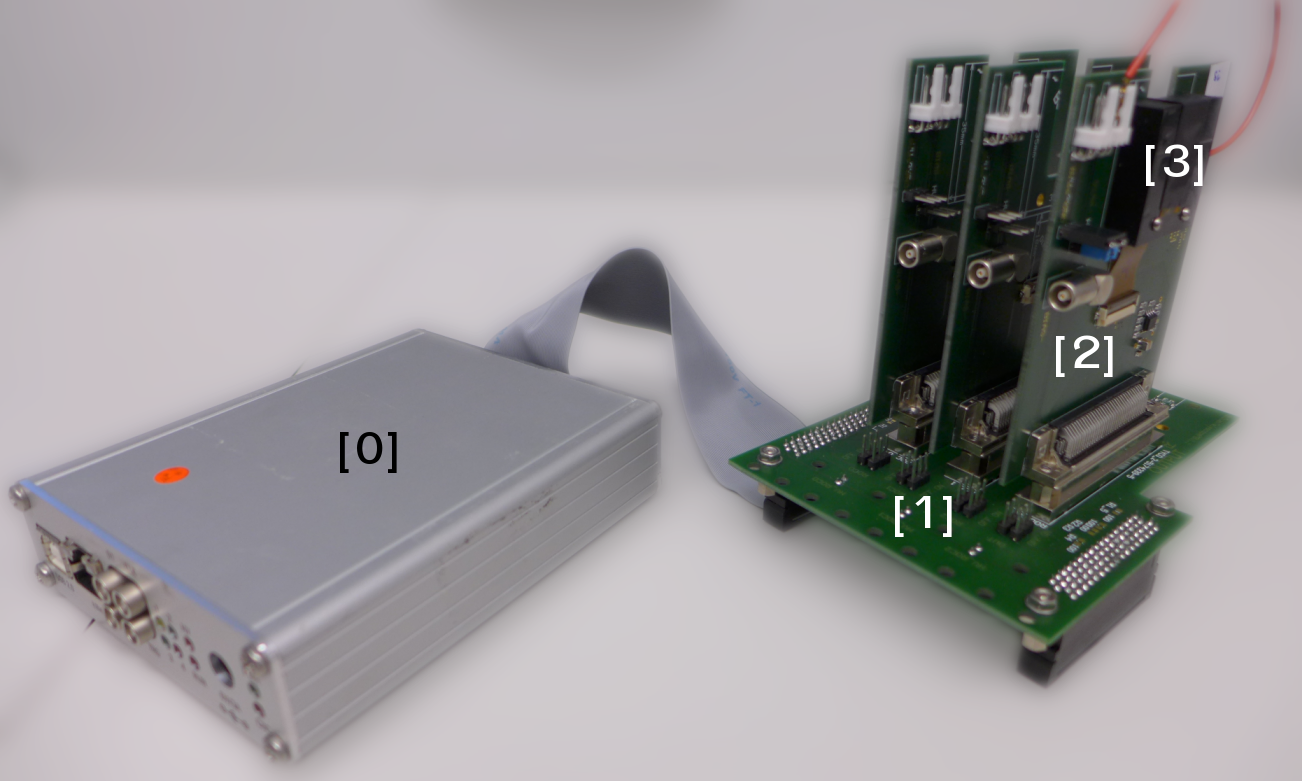
\includegraphics[width=7.8cm]{Pics/TelModule}
	\end{figure}
	\begin{itemize}
		\item $[0]$ Digital Test Board (DTB): interface to a computer
		\item $[1]$ Motherboard: main frame of the telescope
		\item $[2]$ Adaptor Planes: interface to the single pixel chips
		\item $[3]$ CMS Pixel Chip
	\end{itemize}
\end{frame}
% ===================== FRAME 8 ===========================================
\begin{frame}{Telescope Parts}
	\begin{figure} 
		\begin{center}
			\begin{subfigure}{0.48\textwidth}  
				\centering 
				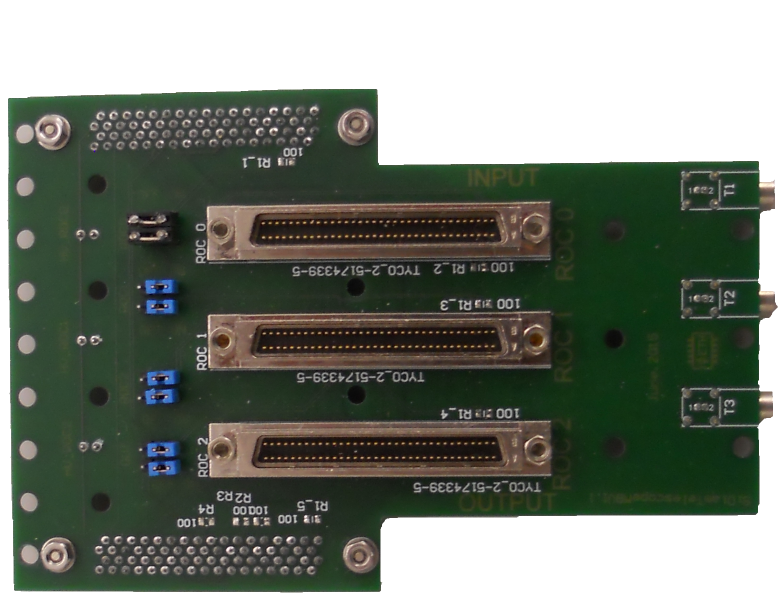
\includegraphics[height=.53\textheight]{Motherboard}
				\caption{motherboard}
			\end{subfigure}
			\begin{subfigure}{0.48\textwidth} 
				\centering 
				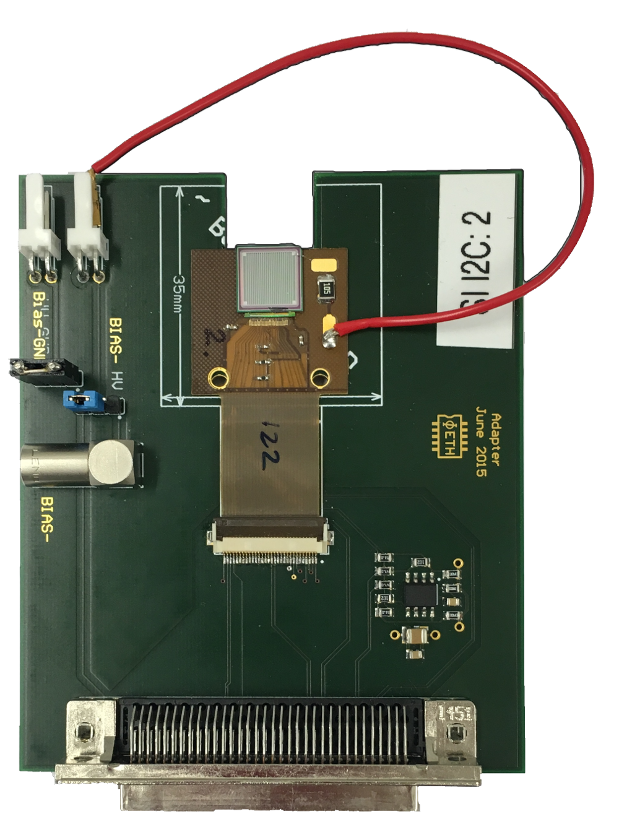
\includegraphics[height=.53\textheight]{Adapter}
				\caption{adaptor plane with pixel chip} 	
			\end{subfigure} 
		\end{center}
	\end{figure}
	\vspace*{5pt}
	\begin{itemize}
		\item up to 3 adaptor plane can be mounted on a single motherboard
		\item \textcolor{red}{\textbf{NEW:}} electrical design of both \ra fixing small bugs from version 1
	\end{itemize}
\end{frame}
% ===================== FRAME 9 ===========================================
\begin{frame}{Telescope Parts}
	\begin{figure} 
		\begin{center}
			\begin{subfigure}{0.4\textwidth}  
				\centering 
				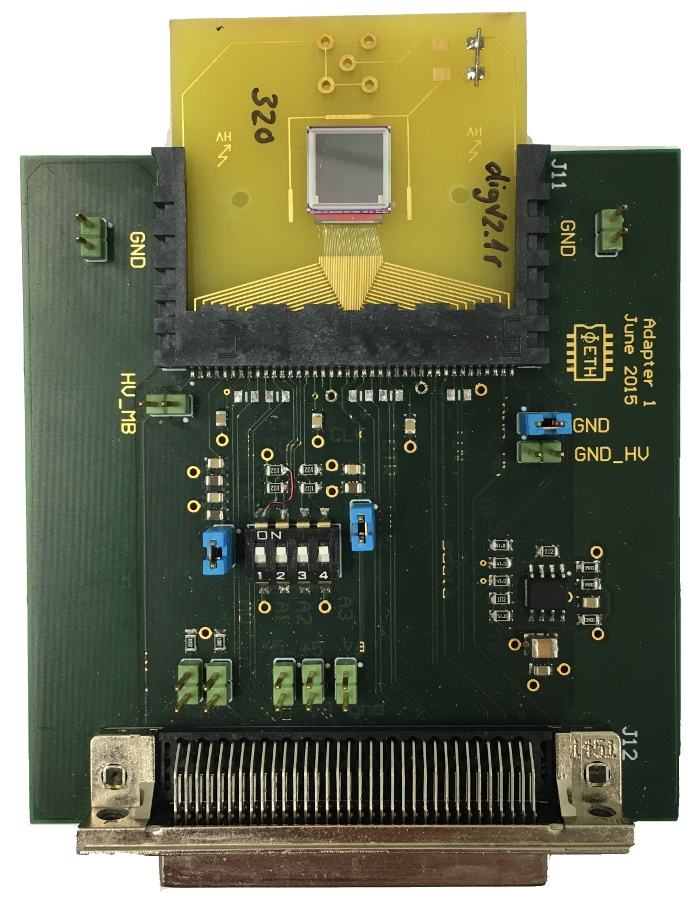
\includegraphics[height=.53\textheight]{DigPlane}
				\caption{digital adaptor plane}
			\end{subfigure}
			\begin{subfigure}{0.28\textwidth} 
				\centering 
				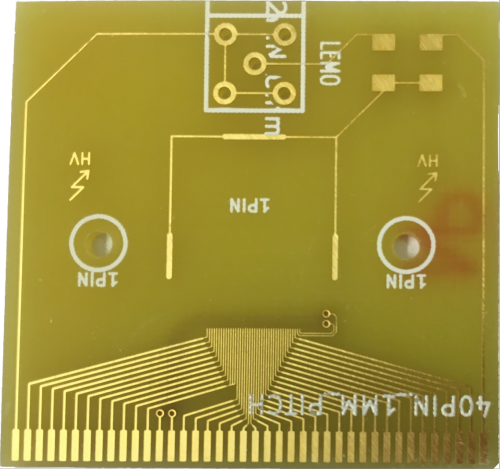
\includegraphics[height=.3\textheight]{CarBoardFront}
				\caption{carrier board front} 	
			\end{subfigure} 
			\begin{subfigure}{0.28\textwidth} 
				\centering 
				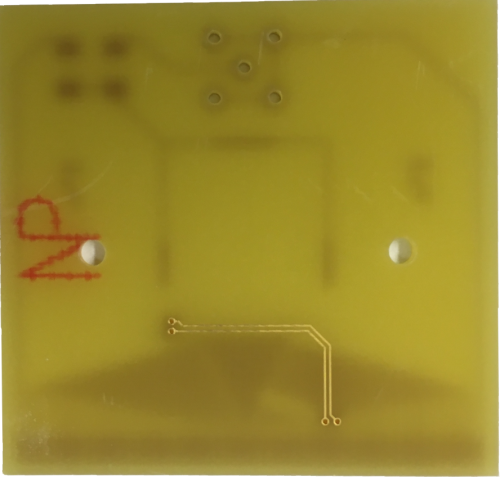
\includegraphics[height=.3\textheight]{CarBoardBack}
				\caption{back} 	
			\end{subfigure} 
		\end{center}
	\end{figure}
	\vspace*{5pt}
	\begin{itemize}
		\item redesigning carrier board for digital pixel chip
		\begin{itemize}
			\item using fast-OR trigger of the newest version of the CMS Pixel Chip (pROC600)
		\end{itemize}
	\end{itemize}
\end{frame}
% ============================ FRAME 10 ==========================================>
\subsection{Setup}
\begin{frame}{Telescope Schematics}
	\only<1>{
		\begin{figure}
			\centering
			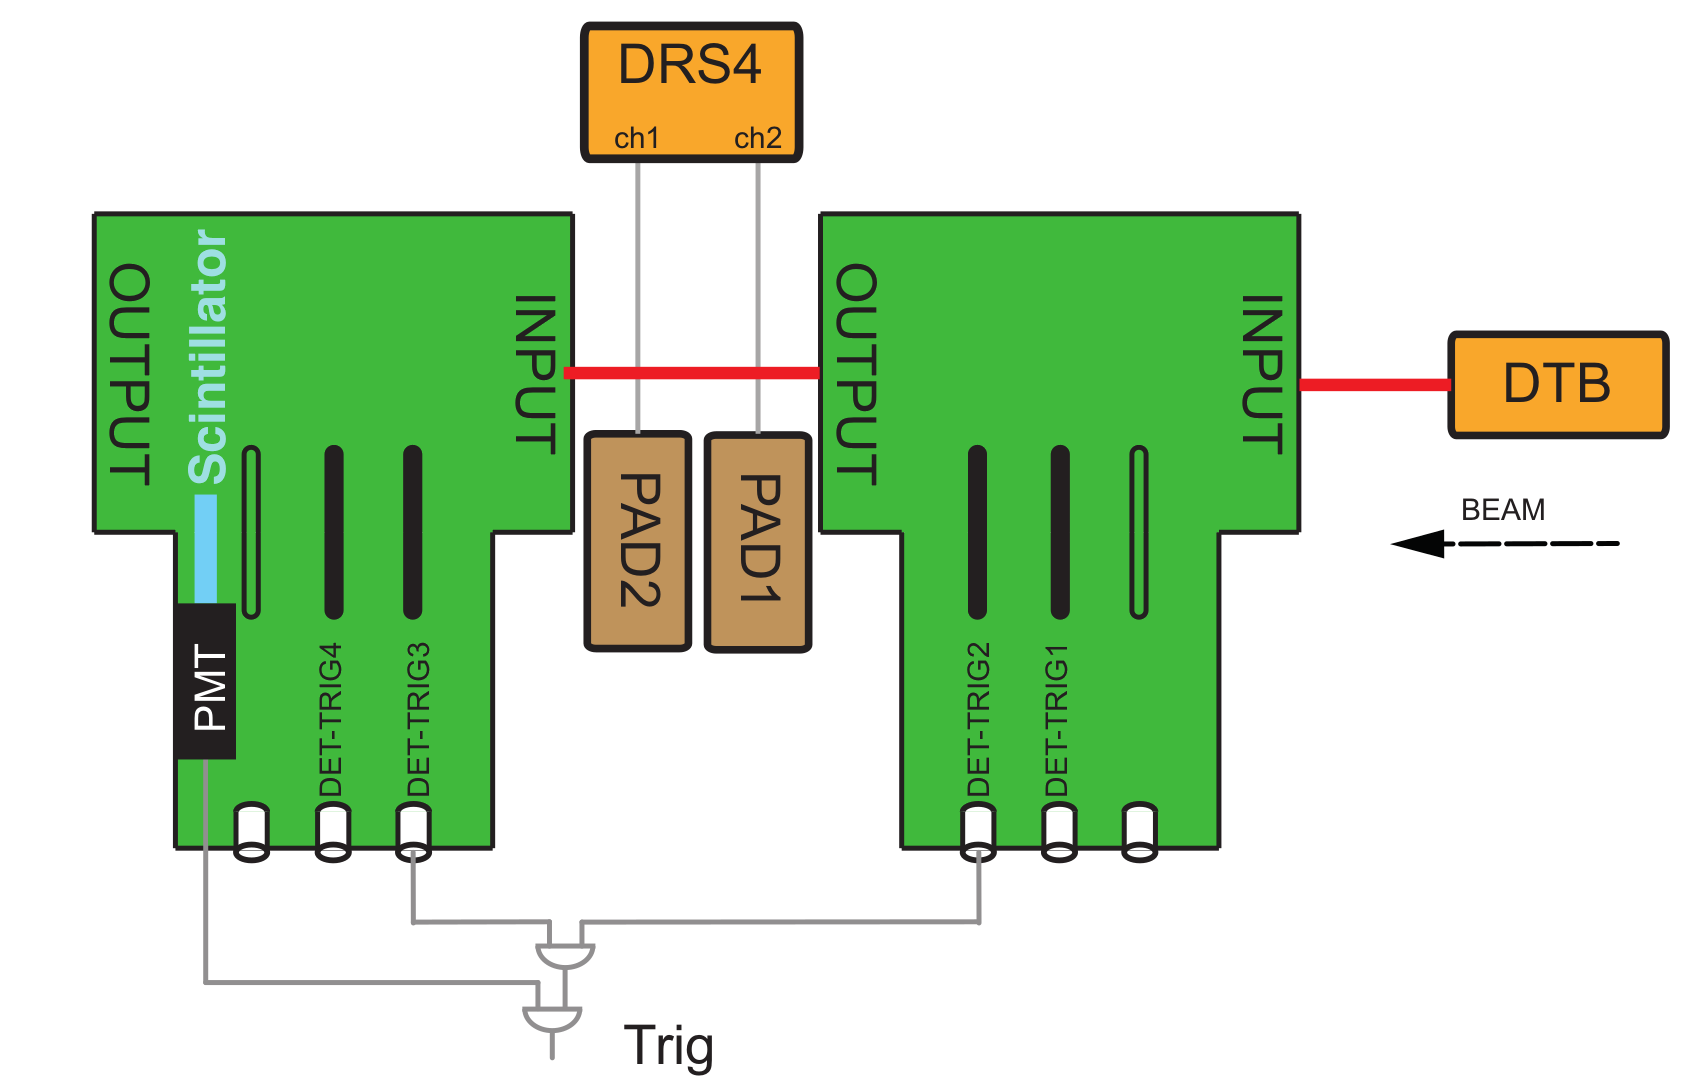
\includegraphics[height=.55\textheight]{TelSchemePad}
			\caption{pad setup}
		\end{figure}}
	\only<2>{
		\begin{figure}
			\centering
			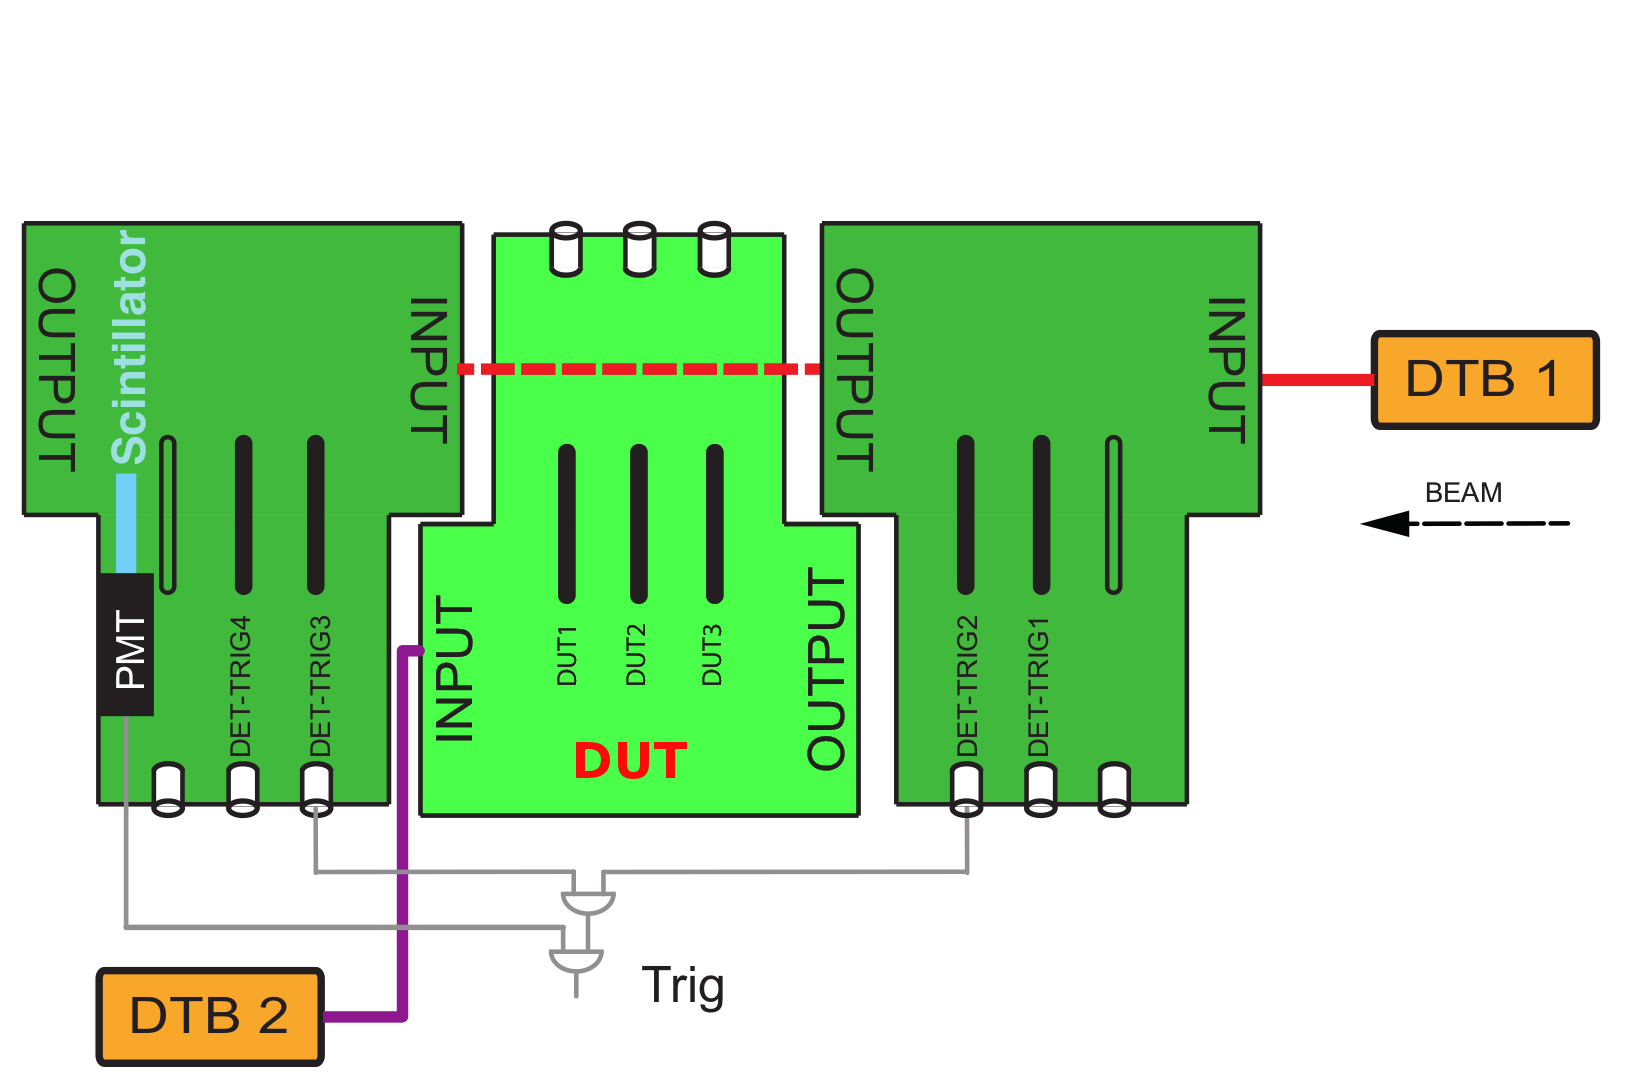
\includegraphics[height=.55\textheight]{TelSchemePix}
			\caption{pixel setup}
		\end{figure}}
	\vspace*{-15pt}
	\begin{itemize}
		\setlength{\itemsep}{\fill}
		\only<1>{\item using PSI DRS4 Evaluation Board as digitizer for the pad waveforms}
		\only<2>{\item using independent telescope module as DUT}
		\item using Digital Test Board (DTB) and pXar software for the telescope readout
		\item global trigger as coincidence of fast-OR self trigger and scintillator signal
		\item EUDAQ as DAQ framework
	\end{itemize}
\end{frame}
% ============================ FRAME 11 ==========================================>
\subsection{Mounting Frame}
\begin{frame}{Mounting Frame}
	\only<1>{
		\begin{figure}
			\centering
			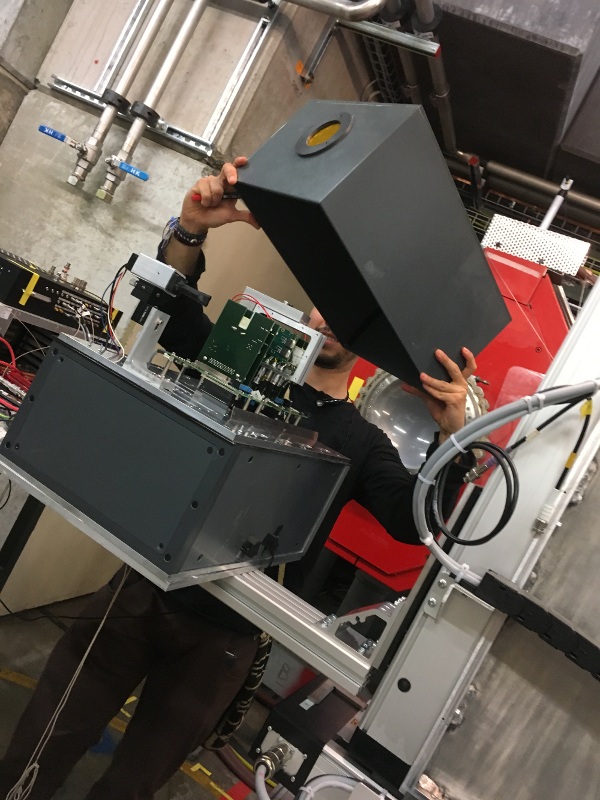
\includegraphics[height=.55\textheight]{Mount1}
		\end{figure}}
	\only<2>{
		\begin{figure}
			\centering
			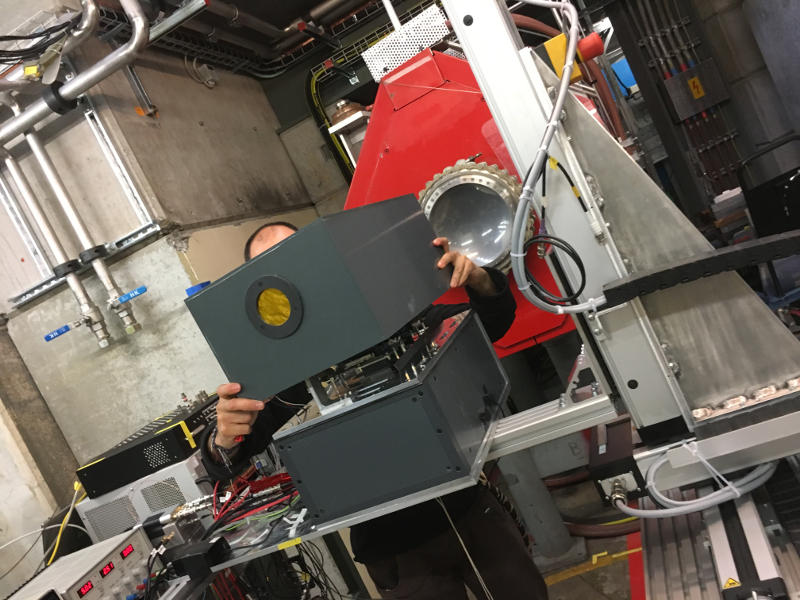
\includegraphics[height=.55\textheight]{Mount2}
		\end{figure}}
	\only<3>{
		\begin{figure}
			\centering
			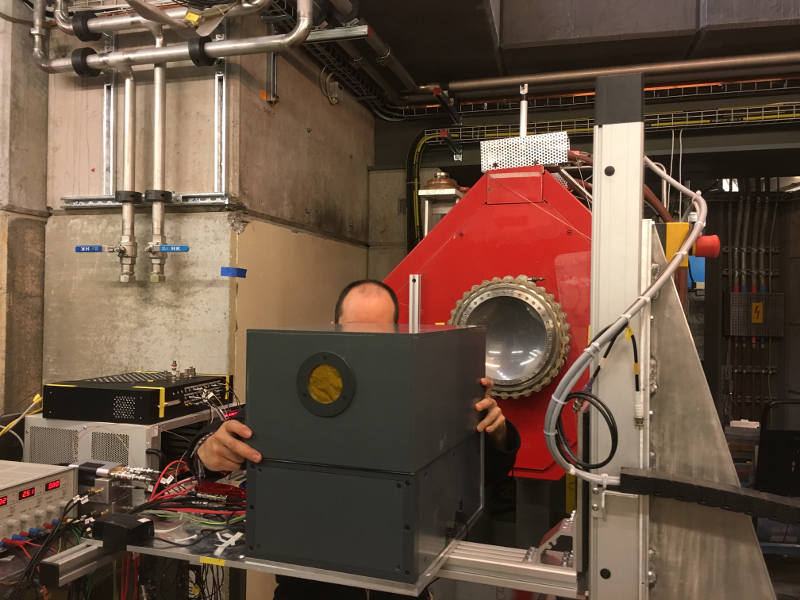
\includegraphics[height=.55\textheight]{Mount3}
		\end{figure}}
	\begin{itemize}
		\setlength{\itemsep}{\fill}
		\item building completely new mounting frame
		\item all cables and some electronics stored inside the box underneath
		\item absolute light tight setup \ra removing all single covers from the detectors
	\end{itemize}
\end{frame}
